\documentclass[11pt]{article}
\usepackage[margin=2.5cm]{geometry}
\usepackage{amsmath,amssymb}
\usepackage{enumitem}
\usepackage{tikz}

\title{\textbf{Rigid Body Dynamics via Lagrange Multipliers}\\[2pt]
\large A solid cylinder rolling without slipping down an inclined plane}
\author{Analytical Mechanics -- Problem Set}
\date{}

\begin{document}
\maketitle

\section*{1. Statement}

A homogeneous solid cylinder of mass $M$ and radius $R$ (moment of inertia about its
axis $I = \tfrac{1}{2}MR^{2}$) rolls without slipping down a plane inclined at an
angle $\alpha$ with respect to the horizontal. Gravity $g$ acts vertically downward.

Let $x(t)$ be the displacement of the center of mass $C$ measured along the plane
(positive downhill), and let $\theta(t)$ be the rotation angle about the cylinder
axis, with the sign chosen so that rolling down corresponds to $\dot\theta > 0$.
The contact is rough enough to prevent slipping, but friction is an
\emph{unknown} static constraint force: do not assume Coulomb's law except where
explicitly requested.

The configuration is described by $q = (x,\theta)$ and the no-slip condition
\[
  \dot x - R\dot\theta = 0 ,
\]
which, being integrable, is equivalent to the holonomic constraint
\[
  \phi(x,\theta) \;=\; x - R\theta \;=\; \text{const.}
\]

Recall the \emph{Lagrange equations of the first kind} for constraints
$\phi_k(q)=0$:
\[
  \frac{d}{dt}\!\left(\frac{\partial L}{\partial \dot q_i}\right)
  - \frac{\partial L}{\partial q_i}
  \;=\; \sum_{k} \lambda_k \,\frac{\partial \phi_k}{\partial q_i},
  \qquad \phi_k(q) = 0 ,
\]
where the multipliers $\lambda_k$ are determined together with the motion and
turn out to be precisely the generalized constraint forces.

\begin{figure}[ht]
  \centering
  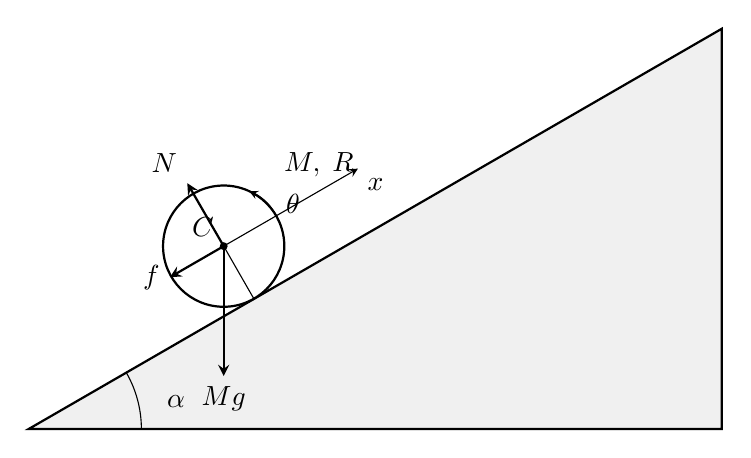
\begin{tikzpicture}[scale=1.1, >=stealth]
    % Inclined plane
    \draw[thick, fill=gray!12] (0,0) -- (8,0) -- (8,4.62) -- cycle;
    \draw (1.3,0) arc[start angle=0, end angle=30, radius=1.3];
    \node at (1.7,0.32) {$\alpha$};
    % Cylinder
    \coordinate (C) at (2.25,2.11);
    \coordinate (P) at (2.60,1.50);
    \draw[thick, fill=white] (C) circle (0.7);
    \fill (C) circle (1.3pt);
    \draw[thin] (C) -- (P);
    \node[above left] at (C) {$C$};
    \node at (3.35,3.05) {$M,\;R$};
    % Coordinates
    \draw[->] (C) -- ++(1.55,0.895) node[below right] {$x$};
    \draw[->] (2.95,2.11) arc[start angle=0, end angle=65, radius=0.7];
    \node at (3.05,2.60) {$\theta$};
    % Forces
    \draw[->, thick] (C) -- ++(0,-1.5) node[below] {$Mg$};
    \draw[->, thick] (C) -- ++(-0.42,0.727) node[above left] {$N$};
    \draw[->, thick] (C) -- ++(-0.62,-0.358) node[left] {$f$};
  \end{tikzpicture}
  \caption{Solid cylinder rolling without slipping down an incline.}
\end{figure}

\section*{2. Questions}

\begin{enumerate}[label=(\alph*), leftmargin=*]
  \item Write the kinetic energy $T$, the potential energy $V$ (taking $V=0$ at
        the initial position), and the Lagrangian
        $L(x,\theta,\dot x,\dot\theta)=T-V$.

  \item Write the two Euler--Lagrange equations of the first kind for this
        system, including the Lagrange multiplier $\lambda$ associated with the
        constraint $\phi = x - R\theta = \text{const}$, together with the
        constraint equation itself.

  \item Solve the system. Obtain the linear acceleration $\ddot x$, the angular
        acceleration $\ddot\theta$, and the multiplier $\lambda$. With initial
        conditions $x(0)=\dot x(0)=\theta(0)=\dot\theta(0)=0$, give
        $x(t)$ and $\theta(t)$.

  \item \textbf{Physical meaning of the multiplier.} Show that $\lambda$ is the
        $x$-component of the static friction force $f$ acting on the cylinder at
        the contact point, and give its magnitude and direction. Compute the
        normal force $N$, and determine the critical angle $\alpha_c$ beyond
        which rolling gives way to slipping if the coefficient of static
        friction is $\mu_s$ (i.e.\ impose $|f| \le \mu_s N$).

  \item Show that along the constrained motion
        $\dot E = \lambda\,(\dot x - R\dot\theta)$, where
        $E = T+V$, and conclude that the mechanical energy is conserved.
        Comment on why the constraint force does no work (ideal constraint,
        d'Alembert's principle).

  \item \textbf{Challenge (system of two rigid bodies).} Replace the fixed
        plane by a wedge of mass $M_w$ that can slide without friction along a
        horizontal table, its face making the same angle $\alpha$. Using the
        generalized coordinates $q = (X, x, \theta)$, where $X$ locates the
        wedge and $x$ the displacement of the cylinder's axis along the face:
        (i) write the Lagrangian and the rolling constraint;
        (ii) obtain $\ddot X$, $\ddot x$, $\ddot\theta$ and $\lambda$;
        (iii) explain why the two normal forces (table--wedge and
        wedge--cylinder) do \emph{not} appear as multipliers in this coordinate
        choice, and indicate how to enlarge the coordinate set with additional
        holonomic constraints so that they do.
\end{enumerate}

\section*{3. Results for self-check}

\begin{itemize}[leftmargin=*]
  \item[(c)] $\displaystyle \ddot x = \frac{g\sin\alpha}{1 + I/(MR^{2})}
             = \frac{2}{3}\,g\sin\alpha$, \quad
             $\displaystyle \ddot\theta = \frac{2g\sin\alpha}{3R}$, \quad
             $\displaystyle \lambda = -\frac{1}{3}Mg\sin\alpha$; \quad
             $x(t) = \tfrac{1}{3}g\sin\alpha\, t^{2}$,
             $\theta(t) = \tfrac{g\sin\alpha}{3R}\, t^{2}$.
  \item[(d)] $f = |\lambda| = \tfrac{1}{3}Mg\sin\alpha$, directed \emph{up} the
             incline (hence the sign of $\lambda$); $\;N = Mg\cos\alpha$;
             slipping begins when $\tan\alpha > 3\mu_s$, i.e.
             $\alpha_c = \arctan(3\mu_s)$.
  \item[(e)] $\displaystyle E = \frac{1}{2}\Bigl(M + \frac{I}{R^{2}}\Bigr)\dot x^{2}
             - Mg\,x\sin\alpha = \text{const}$, since
             $\dot E = \lambda(\dot x - R\dot\theta) = 0$.
\end{itemize}

\end{document}
